\documentclass[
    ngerman,%globale Übergabe der Hauptsprache
%	logofile=example-image, %Falls die Logo Dateien nicht vorliegen
    authorontitle=true,
]{bfhbeamer}


%\usepackage[main=ngerman]{babel}

% Der folgende Block ist nur bei pdfTeX auf Versionen vor April 2018 notwendig
\usepackage{iftex}
\ifPDFTeX
\usepackage[utf8]{inputenc}
\usepackage{blkarray}
\usepackage{array}
\usepackage{graphicx}
\usepackage{biblatex}
\usepackage{amssymb}
\usepackage{amsmath}
\usepackage{mathtools}
\usepackage{hyperref}
\usepackage{beamerbasenotes}%kompatibilität mit TeX Versionen vor April 2018
\fi


\title{TraceSentry}
\subtitle{AI-Aided Caches-n-Logs Monitoring-n-Wiping Daemon}
\author[L. Ammann, J. Scherer, L. Scherer]{Luca Ammann, Janic Scherer, Luca Scherer}
\date{8. Januar 2025}
\institute{BFH-TI}
\titlegraphic*{
\includegraphics{assets/presentation/title}}%is only used with BFH-graphic and BFH-fullgraphic

% Activate the output of a frame number:
\setbeamertemplate{page number in head/foot}[framenumber]

\begin{document}

    \setbeamertemplate{title page}[BFH-graphic]
    \maketitle

    \begin{frame}{Inhalt}
        \framesubtitle{Übersicht}
        \tableofcontents
    \end{frame}


    \section{Problemstellung}\label{sec:problemstellung}
    \setbeamertemplate{Problemstellung}[BFH-ruled]
    \frame{\sectionpage}

    \begin{frame}{Problemstellung}
        \framesubtitle{Problem}
        \begin{itemize}
            \item Cache- und Logdateien: Dateien von \textbf{Betriebssystemen} und \textbf{Anwendungen}.
            \item Viele Benutzer wissen nicht:
            \begin{itemize}
                \item \textbf{Welche} und \textbf{wie viele} Dateien existieren.
                \item Welche Anwendungen diese \textbf{manipulieren}.
            \end{itemize}
            \item Risiken: Datenschutzprobleme und fehlende Kontrolle.
        \end{itemize}
    \end{frame}

    \begin{frame}{Problemstellung}
        \framesubtitle{Avast 2020}
        \begin{center}
            
\includegraphics[width=0.5\textwidth]{assets/presentation/avast-logo}
        \end{center}
        \footnote{\url{https://www.cbsnews.com/news/ftc-avast-browsing-data-privacy/}}
    \end{frame}

    \begin{frame}{Problemstellung}
        \framesubtitle{Chance}
        \begin{itemize}
            \item Entwickeln einer Software für:
            \begin{itemize}
                \item \textbf{Suche} von Dateien.
                \item \textbf{Monitoring} von Dateien bzgl. deren Erstellung, Veränderung und Löschung.
                \item \textbf{Analyse und Bewertung} von Dateien.
                \item \textbf{Bereinigung} von Dateien.
            \end{itemize}
            \item Nutzung eines KI-Modells für:
            \begin{itemize}
                \item Analyse von \textbf{Struktur} (Syntax) und \textbf{Bedeutung} (Semantik) von Dateien.
                \item Bewertung des Dateiinhalts bzgl.
                dessen \textbf{Schädlichkeit}.
                \item Empfehlungen von nötigen \textbf{Massnahmen}.
            \end{itemize}
        \end{itemize}
    \end{frame}

    \begin{frame}{Projektziel}
        \begin{itemize}
            \item Entwicklung einer \textbf{plattformunabh\"angigen, benutzerfreundlichen} Anwendung mit Dokumentation.
            \item Praxisnahe \textbf{Fallstudie} zur Evaluation des Potentials von aktuellen KI-Technologien.
            \item Fokus auf \textbf{Resultate} und Kernfunktionalit\"at.
        \end{itemize}
    \end{frame}

    \begin{frame}{Rahmenbedingungen}
        \begin{itemize}
            \item Entwicklung eines Hintergrundprozesses (\textbf{Daemon}).
            \item Kommandozeilen-Interface f\"ur Benutzerinteraktion (\textbf{CLI}).
            \item \textbf{Cache- und Log}dateien als prim\"arer Fokus, Erweiterung auf andere Dateitypen m\"oglich.
            \item \textbf{FLOSS-lizenzierte} und \textbf{plattformunabh\"angige} Software.
            \item Evaluation eines aktuellen KI-Modells. \textbf{Keine Eigenentwicklung}.
        \end{itemize}
    \end{frame}


    \section{Lösung}\label{sec:loesung}
    \setbeamertemplate{Lösung}[BFH-ruled]
    \frame{\sectionpage}

    \begin{frame}{Architektur}
        \begin{center}
            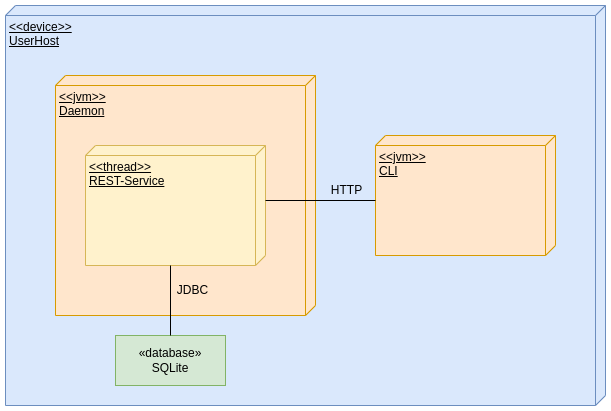
\includegraphics[width=0.7\textwidth]{assets/DeplDiagram-v2}
        \end{center}
    \end{frame}

    \begin{frame}{Der Daemon}
        \framesubtitle{Spring basierter Service}
        \begin{columns}
            \begin{column}{0.7\textwidth}
                \begin{itemize}
                    \item \textbf{Periodisch \& automatisch:} Ausführung von Monitoringaufgaben
                    \begin{itemize}
                        \item Erstellen von Dateisystem-Snapshots (Hashbäume).
                        \item Vergleich von Snapshots (mit Vor- bzw.\ Nachfolger).
                    \end{itemize}
                    \item \textbf{Via REST-API:} Kommunikation mit Benutzer
                    \begin{itemize}
                        \item Suche von Dateien (z.B.\ mit regulären Ausdrücken).
                        \item Management von überwachten Pfaden.
                        \item Operationen auf Snapshots.
                        \item Anfragen von KI-Einschätzungen.
                        \item Löschen von Dateien.
                        \item Administrative Funktionen (Starten/Stoppen des Daemons).
                    \end{itemize}
                \end{itemize}
            \end{column}
            \begin{column}{0.3\textwidth}
                \begin{center}
                    
\includegraphics[width=0.5\textwidth]{assets/presentation/ghost-smile}
                \end{center}
            \end{column}
        \end{columns}
        \note[item]{https://www.svgrepo.com/}

    \end{frame}

    \begin{frame}{Die Kommandozeile}
        \framesubtitle{Spring Shell basierte CLI}
        \begin{columns}
            \begin{column}{0.7\textwidth}
                \begin{itemize}
                    \item \textbf{Warum eine CLI?}
                    \begin{itemize}
                        \item Effizienz bei der Entwicklung.
                        \item Zielgruppe: technisch versierte Benutzer.
                        \item Architektur würde in Zukunft auch eine GUI erlauben.
                    \end{itemize}
                    \item \textbf{Funktionalitäten:}
                    \begin{itemize}
                        \item Parsing und Validierung von Benutzereingaben.
                        \item Kommunikation mit dem Daemon via REST-API\@.
                    \end{itemize}
                \end{itemize}
            \end{column}
            \begin{column}{0.3\textwidth}
                \begin{center}
                    
\includegraphics[width=0.5\textwidth]{assets/presentation/prompt}
                \end{center}
            \end{column}
        \end{columns}
    \end{frame}

    \begin{frame}{Datenbank}
        \framesubtitle{SQLite}
        \begin{columns}
            \begin{column}{0.6\textwidth}
                \begin{itemize}
                    \item File-basiert (serverlos)
                    \item Light-weight
                    \item Kompatibel mit Spring Data (JPA)
                    \begin{itemize}
                        \item JDBC-/Hibernate-Kompatibilität
                        \item Transaktionen
                        \item Grundlegende SQL-Funktionen
                        \item etc.
                    \end{itemize}
                \end{itemize}
            \end{column}
            \begin{column}{0.4\textwidth}
                \begin{center}
                    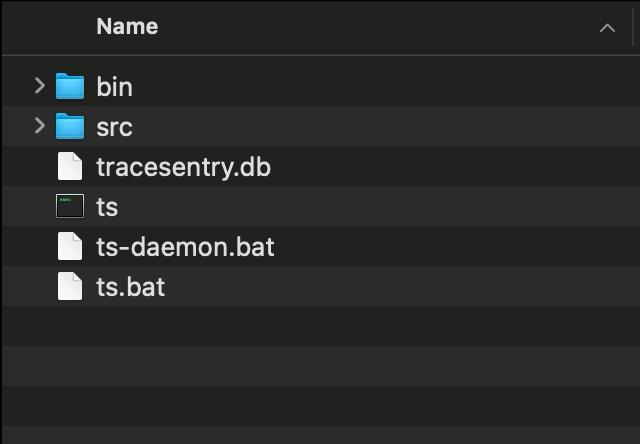
\includegraphics[width=1\textwidth]{assets/presentation/db}
                \end{center}
            \end{column}
        \end{columns}
    \end{frame}

    \begin{frame}{Monitoring (Hashb\"aume)}
        \begin{columns}
            \begin{column}{0.5\textwidth}
                Struktur:
                \begin{itemize}
                    \item Die \textbf{Wurzel} entspricht dem überwachten Pfad.
                    \item \textbf{Innere Knoten} entsprechen Unterverzeichnissen.
                    \item \textbf{Blätter} entsprechen Dateien (oder leeren Verzeichnissen).
                \end{itemize}
                Hashing:
                \begin{align*}
                    B &\coloneqq \text{Blatt} \\
                    N &\coloneqq \text{Nicht-Blatt} \\
                    K &\coloneqq \text{Kind} \\
                    H(B) &= H(Datei)\\
                    H(N) &= H(H(K_1) \|H(K_2) \| \dots \|H(K_k))\\
                \end{align*}
            \end{column}
            \begin{column}{0.5\textwidth}
                \begin{center}
                    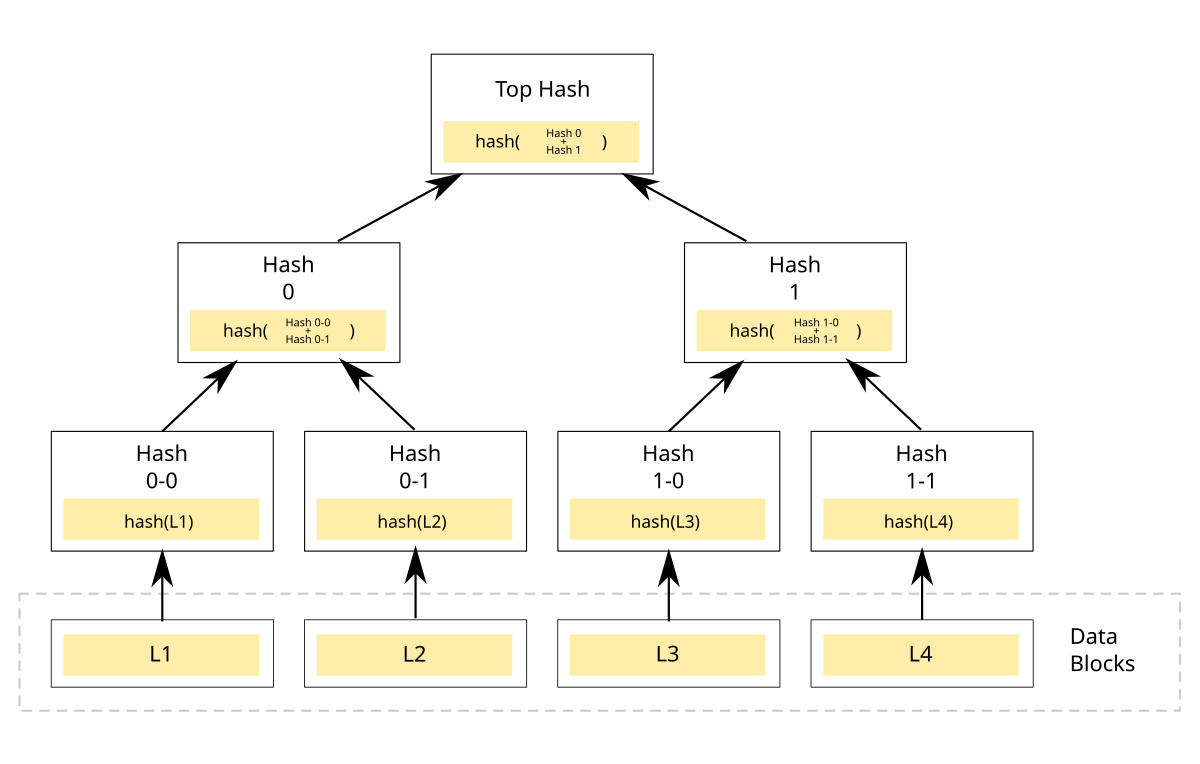
\includegraphics[width=1\textwidth]{assets/presentation/hashtree}
                \end{center}
            \end{column}
        \end{columns}
    \end{frame}

    \begin{frame}{KI-Fallstudie}
        \begin{columns}
            \begin{column}{0.5\textwidth}
                Ziel:\\
                Evaluation des Potentials von aktuellen KI-Technologien im Bereich der Dateianalyse.
            \end{column}
            \begin{column}{0.5\textwidth}
                Vorgehen:
                \begin{itemize}
                    \item Auswahl einer KI-Technologie und eines Modells.
                    \item Generierung von Testdateien.
                    \item Evaluation und Aufbereitung der Resultate.
                \end{itemize}
            \end{column}
        \end{columns}
    \end{frame}


    \section{Demo}\label{sec:demo}
    \setbeamertemplate{Demo}[BFH-ruled]
    \frame{\sectionpage}


    \section{Projektmanagement}\label{sec:projektmanagement}
    \setbeamertemplate{Projektmanagement}[BFH-ruled]
    \frame{\sectionpage}

    \begin{frame}{Rückblick}
        \framesubtitle{Produktziele}
        \begin{columns}
            \begin{column}{0.5\textwidth}
                \begin{tabular}{l|c}
                    \textbf{Ziel}                & \textbf{Erreicht} \\
                    \hline
                    Suche von Dateien            & Ja                \\
                    Periodisches Monitoring      & Ja                \\
                    Datei-Bereinigung            & Ja                \\
                    Plattformunabhängig          & Ja                \\
                    Modular und erweiterbar      & Ja                \\
                    Automatische Testabdeckung   & Ja                \\
                    AI-Einbindung mit Fallstudie & Ja                \\
                \end{tabular}\par
            \end{column}
            \begin{column}{0.5\textwidth}
                
\includegraphics[width=1\textwidth]{assets/presentation/goals}
            \end{column}
        \end{columns}
    \end{frame}

    \begin{frame}{Retro}
        \framesubtitle{Erfahrungen und Erkenntnisse}
        \begin{center}
            \begin{columns}[t]
                \begin{column}{0.3\textwidth}
                    \textbf{Rollen und Stakeholder}
                    \begin{itemize}
                        \item Arbeitsaufteilung
                        \item Kommunikation
                    \end{itemize}
                \end{column}


                \begin{column}{0.4\textwidth}
                    \textbf{Scrum Events und Artifacts}
                    \begin{itemize}
                        \item Retro, Review, Planning
                        \item Sprint
                        \item Velocity/Burn-Down-Chart
                    \end{itemize}
                \end{column}

            \end{columns}
        \end{center}
    \end{frame}


    \section{Fazit}\label{sec:fazit}
    \setbeamertemplate{Fazit}[BFH-ruled]
    \frame{\sectionpage}

    \begin{frame}{Fazit}
        \begin{itemize}
            \item Alle definierten \textbf{Ziele und Lieferobjekte} wurden erreicht.
            \item Viel gelernt, insbesondere in den Bereichen \textbf{Projektmanagement und Technologien}.
            \item \textbf{Potential} von aktuellen KI-Technologien sowie unserer Software wurde aufgezeigt.
        \end{itemize}
    \end{frame}


    \section{Ausblick}\label{sec:ausblick}
    \setbeamertemplate{Ausblick}[BFH-ruled]
    \frame{\sectionpage}

    \begin{frame}{Zukünftige Arbeiten}
        \begin{itemize}
            \item Schlussfolgerungen aus Änderungen von Dateien ziehen.
            \item Schreibende Prozesse erkennen.
            \item Höhere Dateikompatibilität.
            \item Evaluation von dedizierten KI-Modellen für Anomalieerkennung.
        \end{itemize}
    \end{frame}

    \begin{frame}{Fragen}
        \begin{center}
            
\includegraphics[width=0.4\textwidth]{assets/presentation/questions_frame_image}
        \end{center}
    \end{frame}
\end{document}
